% !TEX root = ../main.tex
% --+ 20.15a Q2 +---------------------------------------------------------------
\begin{frame}{Uncorrected DIS $v_z$ Plots: $Q^2$}
    \label{20.15a::q2}

    \begin{figure}[t]
        \centering{
            \fbox{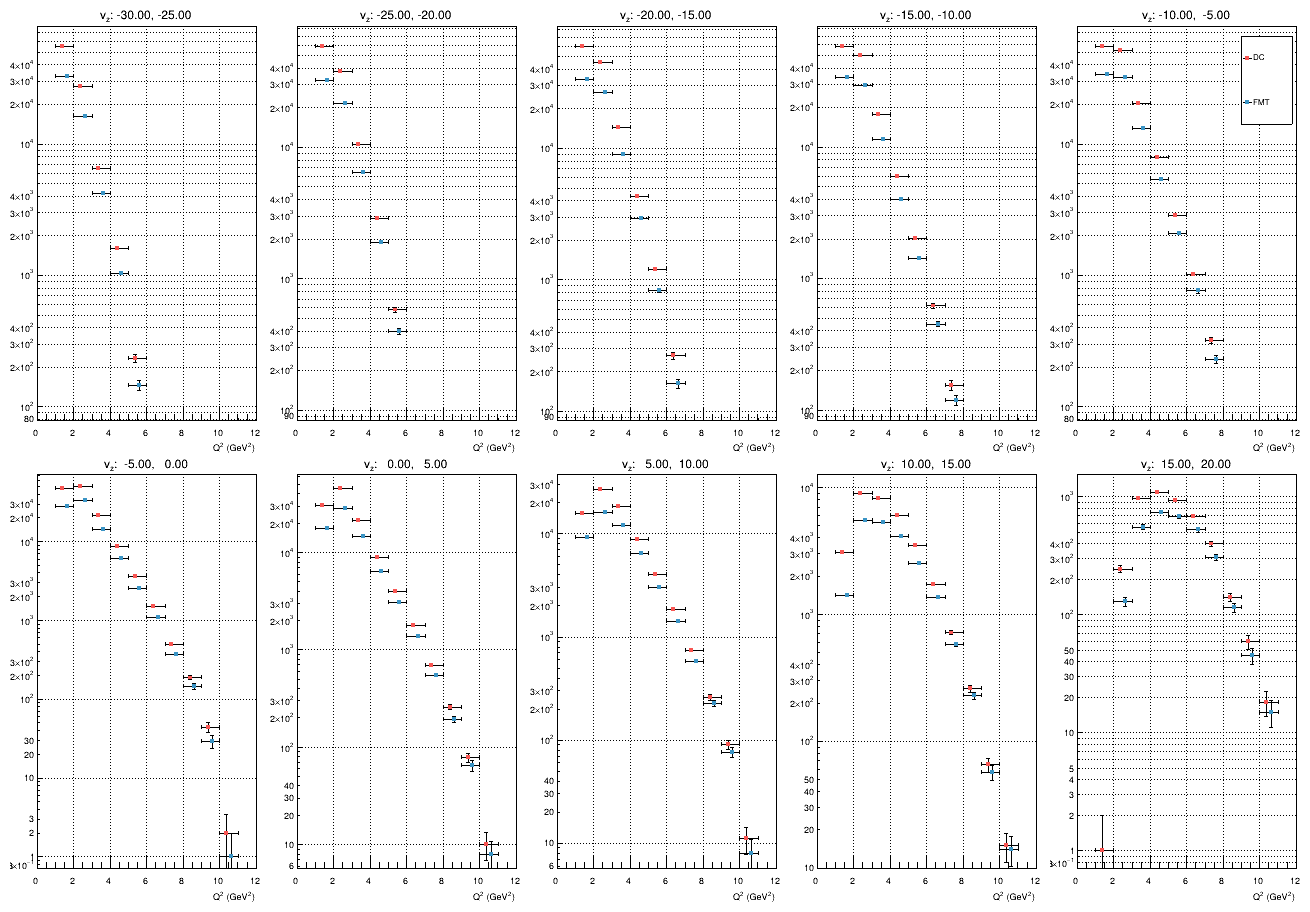
\includegraphics[width=0.72\textwidth]{15a_q2.png}}
        }
    \end{figure}

    \backref{12.12::q2}
\end{frame}

% --+ 20.15b NU +---------------------------------------------------------------
\begin{frame}{Uncorrected DIS $v_z$ Plots: $\nu$}
    \label{20.15b::nu}

    \begin{figure}[t]
        \centering{
            \fbox{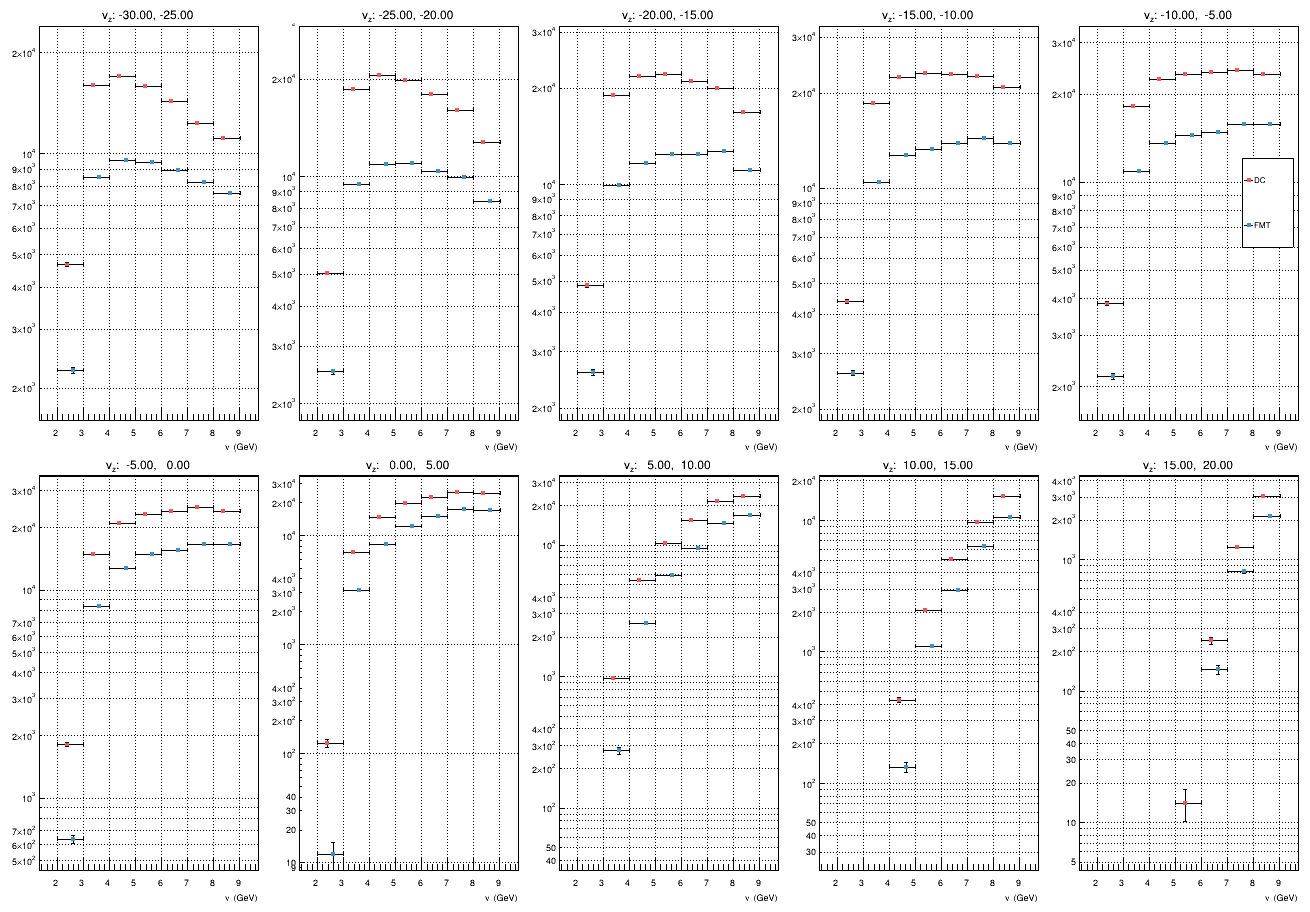
\includegraphics[width=0.72\textwidth]{15b_nu.png}}
        }
    \end{figure}

    \backref{12.13::nu}
\end{frame}

% --+ 20.15c zh pi+ +-----------------------------------------------------------
\begin{frame}{Uncorrected DIS $v_z$ Plots: $z_h$ for $\pi^+$}
    \label{20.15c::zh_pi+}

    \begin{figure}[t]
        \centering{
            \fbox{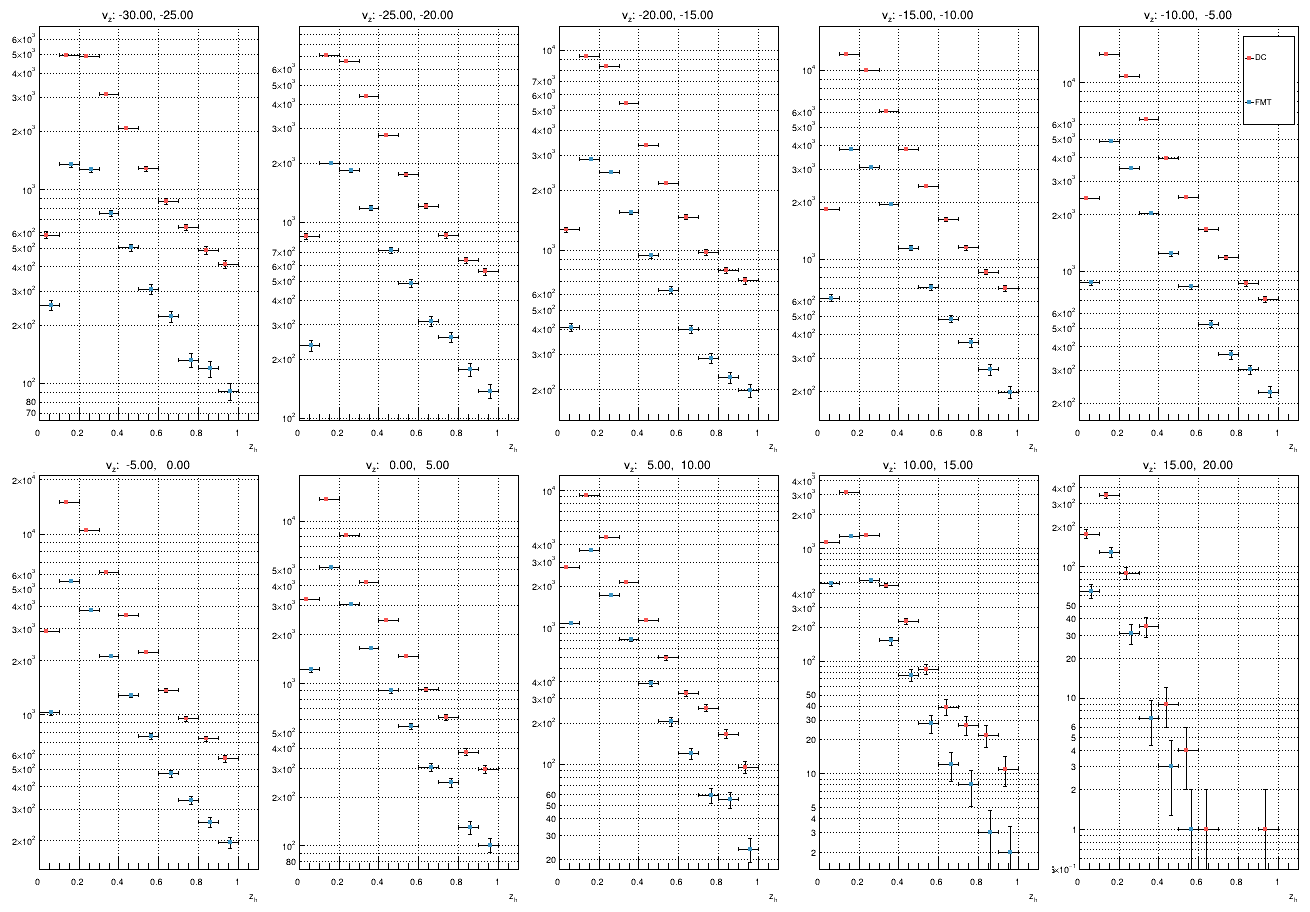
\includegraphics[width=0.72\textwidth]{15c_zh_pi+.png}}
        }
    \end{figure}

    \backref{12.14::zh}
\end{frame}

% --+ 20.15d zh pi- +-----------------------------------------------------------
\begin{frame}{Uncorrected DIS $v_z$ Plots: $z_h$ for $\pi^-$}
    \label{20.15d::zh_pi-}

    \begin{figure}[t]
        \centering{
            \fbox{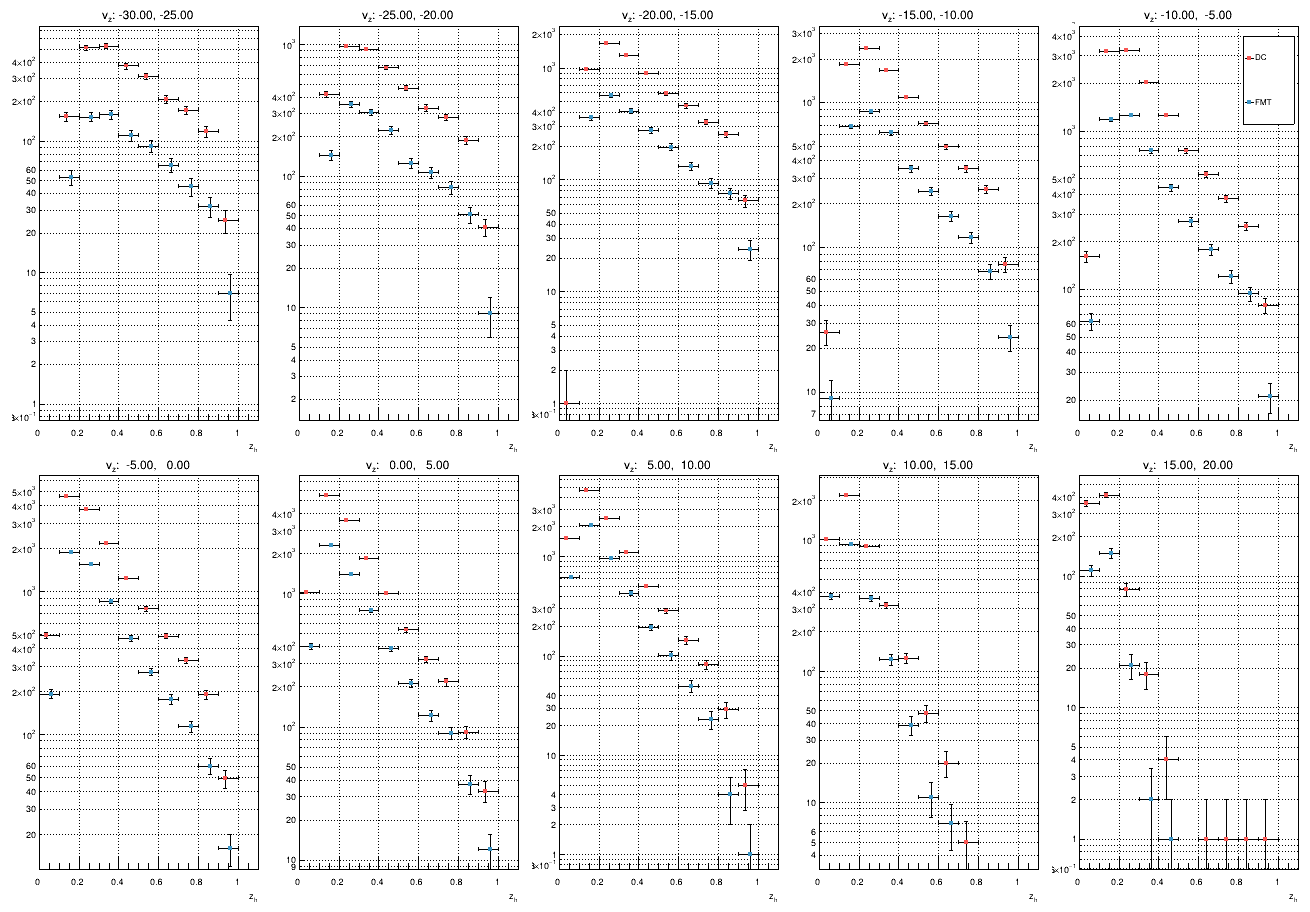
\includegraphics[width=0.72\textwidth]{15d_zh_pi-.png}}
        }
    \end{figure}

    \backref{12.14::zh}
\end{frame}

% --+ 20.15e pt2 pi+ +----------------------------------------------------------
\begin{frame}{Uncorrected DIS $v_z$ Plots: $p_T^2$ for $\pi^+$}
    \label{20.15e::pt2_pi+}

    \begin{figure}[t]
        \centering{
            \fbox{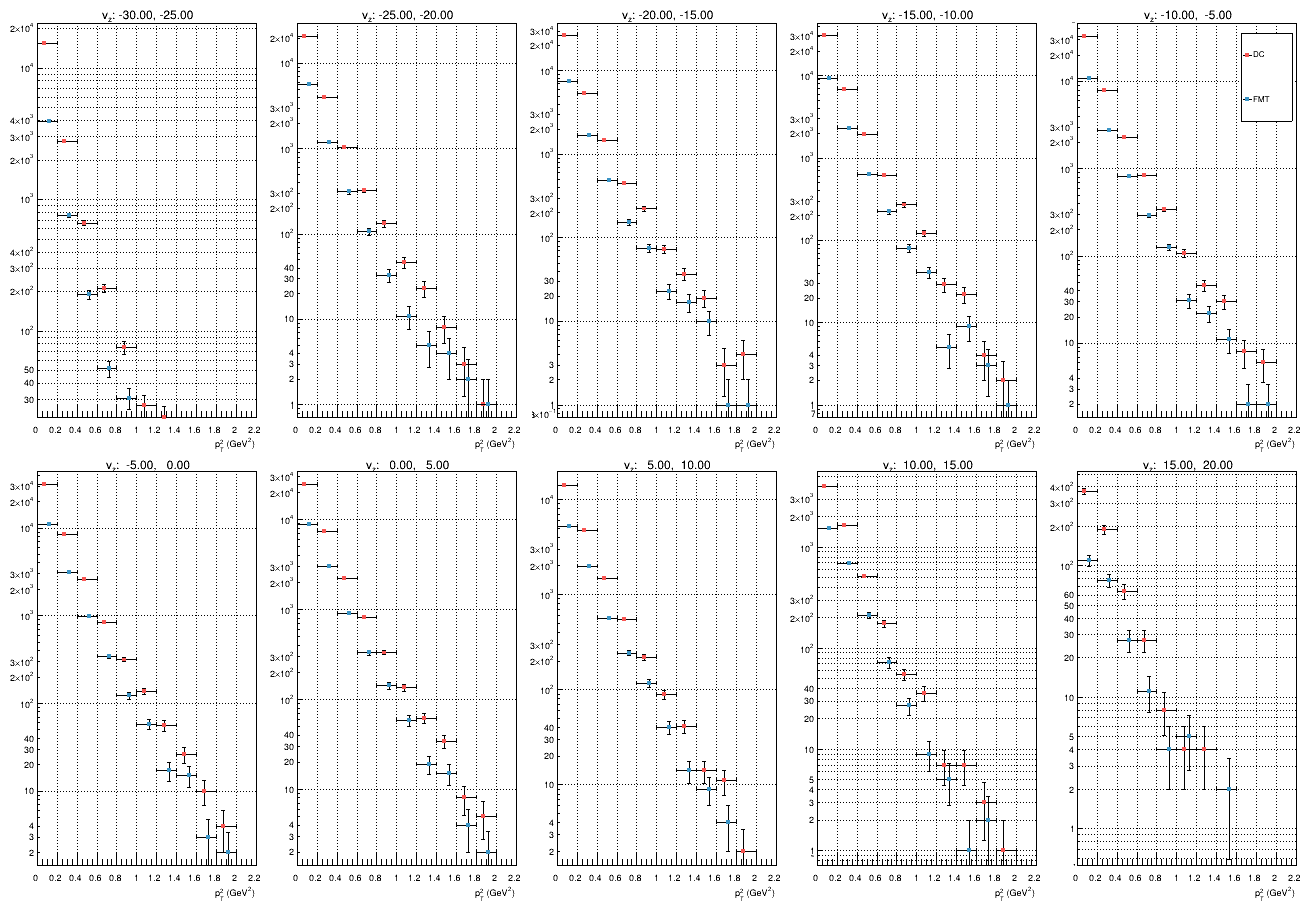
\includegraphics[width=0.72\textwidth]{15e_pt2_pi+.png}}
        }
    \end{figure}

    \backref{12.15::pt2}
\end{frame}

% --+ 20.15f pt2 pi- +----------------------------------------------------------
\begin{frame}{Uncorrected DIS $v_z$ Plots: $p_T^2$ for $\pi^-$}
    \label{20.15f::pt2_pi-}

    \begin{figure}[t]
        \centering{
            \fbox{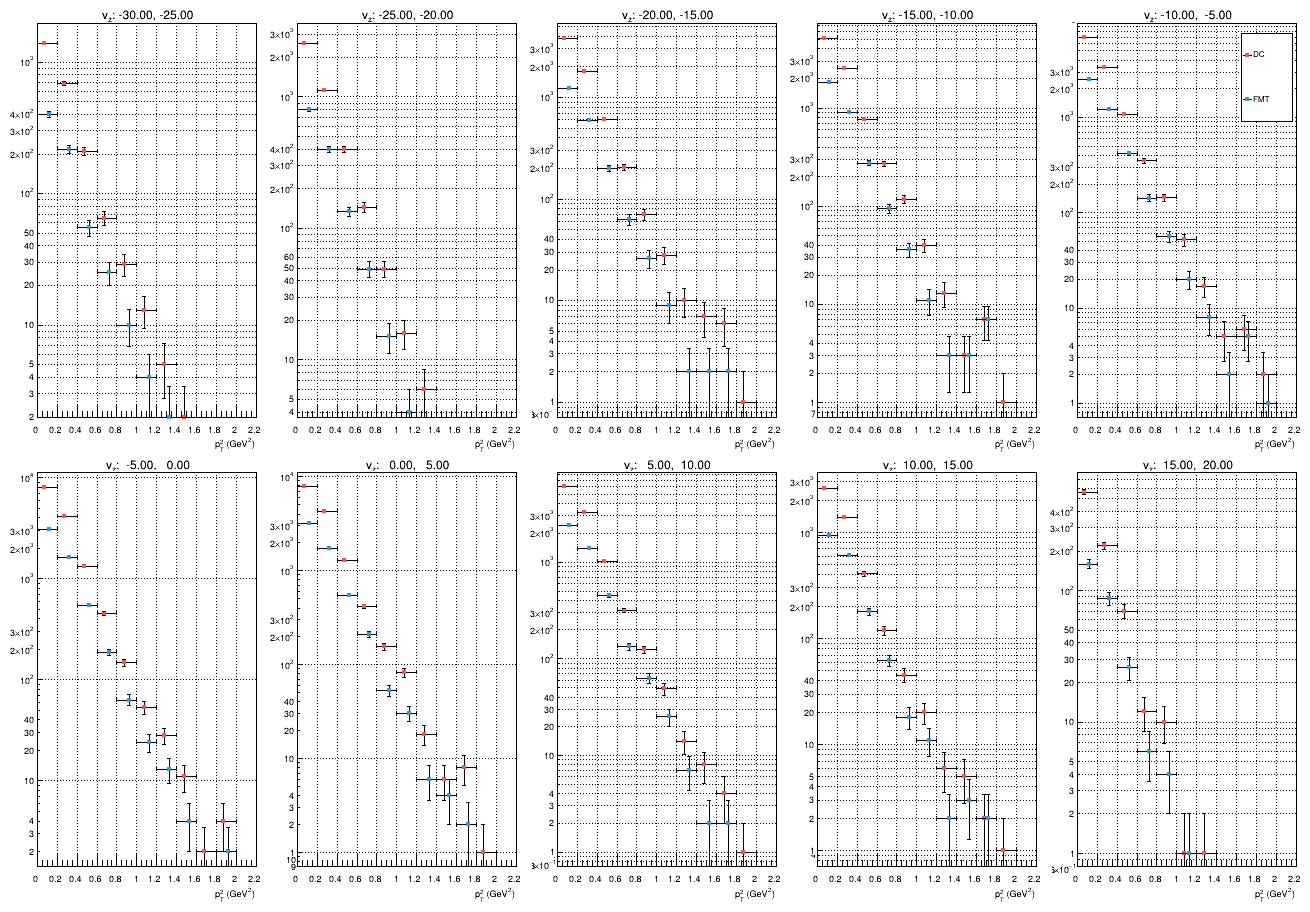
\includegraphics[width=0.72\textwidth]{15f_pt2_pi-.png}}
        }
    \end{figure}

    \backref{12.15::pt2}
\end{frame}

% --+ 20.15g phipq pi+ +--------------------------------------------------------
\begin{frame}{Uncorrected DIS $v_z$ Plots: $\phi_{PQ}$ for $\pi^+$}
    \label{20.15g::phipq_pi+}

    \begin{figure}[t]
        \centering{
            \fbox{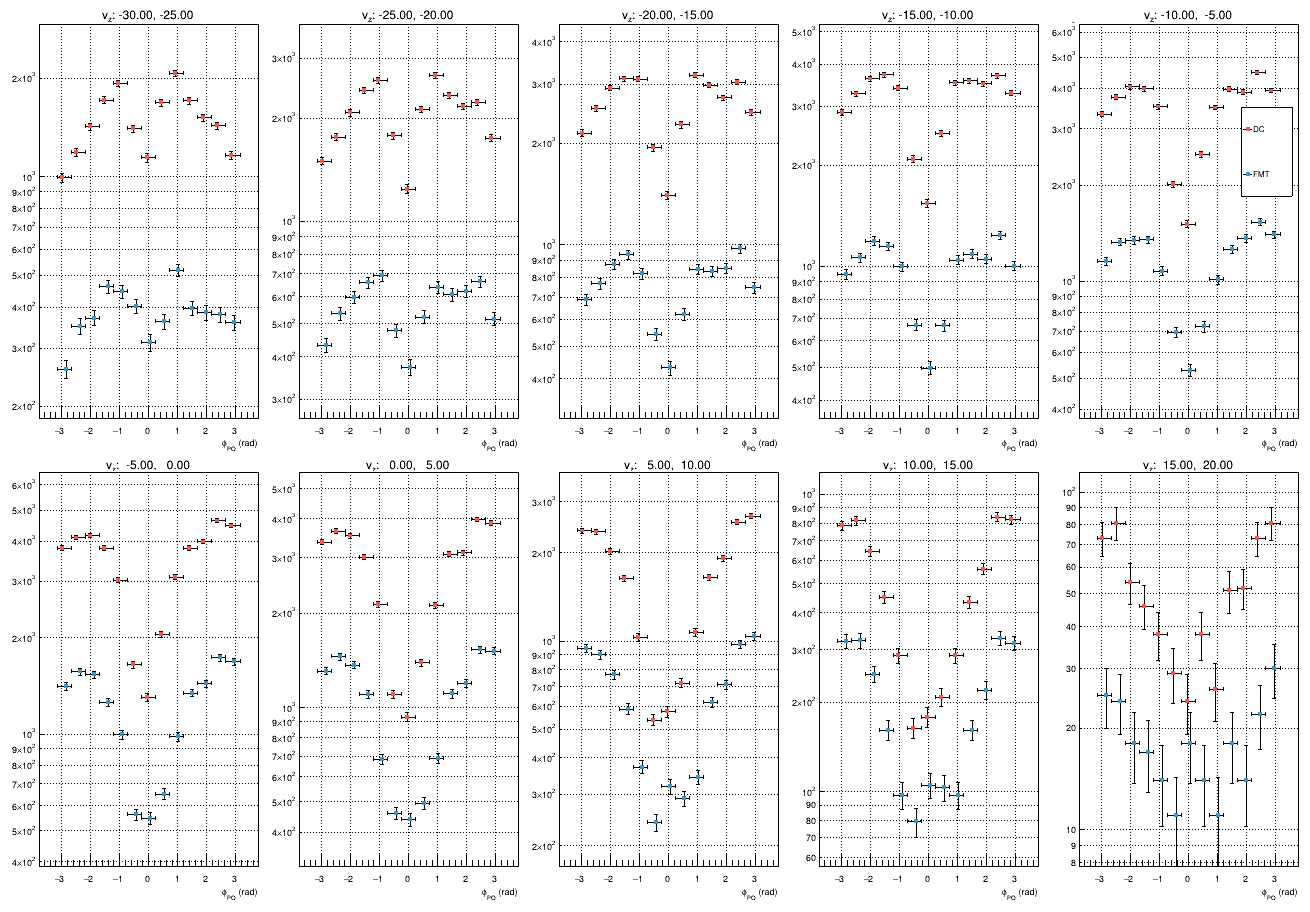
\includegraphics[width=0.72\textwidth]{15g_phipq_pi+.png}}
        }
    \end{figure}

    \backref{12.16::phipq}
\end{frame}

% --+ 20.15h phipq pi- +-----------------------------------------------------------
\begin{frame}{Uncorrected DIS $v_z$ Plots: $\phi_{PQ}$ for $\pi^-$}
    \label{20.15h::phipq_pi-}

    \begin{figure}[t]
        \centering{
            \fbox{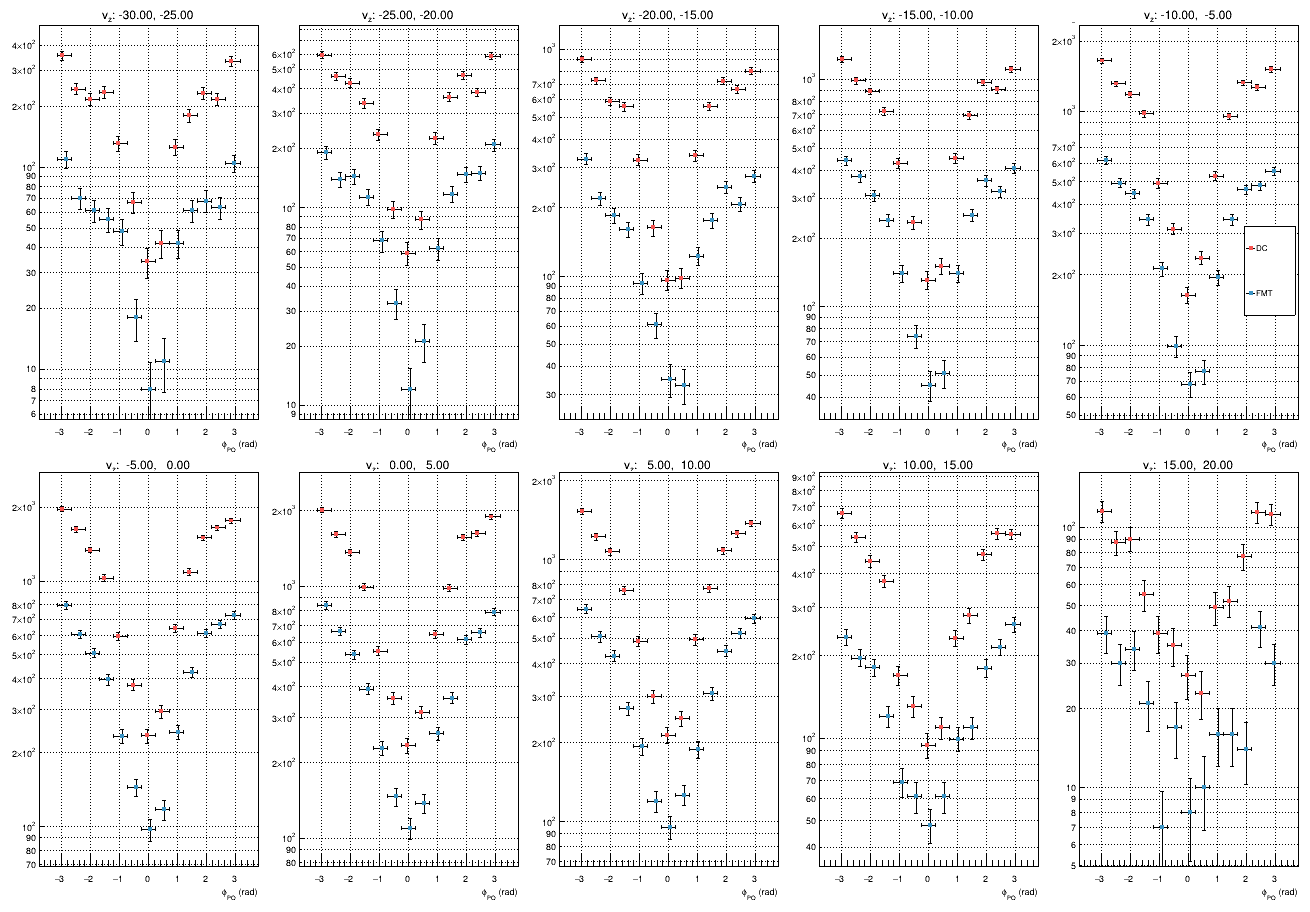
\includegraphics[width=0.72\textwidth]{15h_phipq_pi-.png}}
        }
    \end{figure}

    \backref{12.16::phipq}
\end{frame}
